\documentclass[a4paper,12pt]{article}

% don't forget the document class, generally : \documentclass[a4paper,12pt]{article}

\usepackage[utf8]{inputenc}
\usepackage[french]{babel}
\usepackage{graphicx}
\usepackage{gensymb}
\usepackage{amsmath}
\usepackage{float}
\usepackage{scrextend}
\usepackage{caption} 
\usepackage{siunitx}
\usepackage{enumitem}
\usepackage{amsthm}
\usepackage{fancyhdr}
\usepackage{amssymb}
\usepackage{wrapfig}
\usepackage{geometry}
\usepackage{standalone}
\usepackage{import}
\usepackage[usenames, dvipsnames]{color}

 \usepackage{biblatex} % manages bibliography and references
\addbibresource{sample.bib}


\geometry{hmargin=1in, vmargin=1in}

 \newenvironment{absolutelynopagebreak}
 {\par\nobreak\vfil\penalty0\vfilneg
 \vtop\bgroup}
 {\par\xdef\tpd{\the\prevdepth}\egroup
 \prevdepth=\tpd}
 
 \pagestyle{fancy}                        
\fancyhf{}                               
\fancyhf[HL]{Application des maths}                
\fancyhf[HR]{Géométrie euclidienne}             
\fancyhf[FC]{\thepage/\pageref{Lastpage}}
 
\newtheorem{definition}{Définition}[section]
\newtheorem{theorem}{Théorème}
\newtheorem{corollary}{Corollaire}[theorem]
\newtheorem{lemma}[theorem]{Lemme}
\newtheorem*{hyp}{Hypothèse}
\newtheorem*{concl}{Conclusion}
\newtheorem*{remark}{Remarque}

\captionsetup{format=default,labelformat=simple,labelsep=colon,
justification=justified,font={sf,small},labelfont=bf,
textfont=default} 



\begin{document}

\subsection{Théorème de l'angle externe}
\begin{theorem}
Dans tout triangle et pour chaque sommet, l'angle externe est plus grand que l'angle intérieur en chacun des autres sommets.
\end{theorem}

\begin{proof}
Considérons un triangle $\triangle abc$ qui a $\alpha'$ comme angle externe à $\alpha$.
\begin{figure}[H]
    \centering
    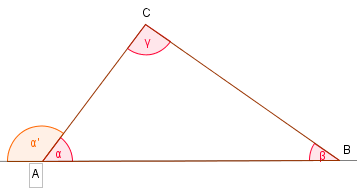
\includegraphics[scale=0.9]{Angle_externe_1.PNG}
\end{figure}

Se présentent alors trois cas possibles :

\begin{enumerate}
    \item $\alpha'  \equiv \gamma$
    \item $\alpha' < \gamma$
    \item $\alpha' > \gamma$
\end{enumerate}
Il nous faut démontrer que les cas 1 et 2 sont impossibles et que seul le cas 3 reste correct.
\begin{enumerate}

    \item Tout d'abord nous reportons le côté $CB$ sur le prolongement du segment $AB$ et obtenons le segment DA. Ensuite, nous relions les points $C$ et $D$. Ainsi nous obtenons un nouveau triangle $\triangle DCA$, dont l'un des angles est $\alpha'$.
	Grâce au premier cas d'isométrie des triangles, on déduit que les triangles $\triangle DCA$ et $\triangle abc$ sont isométriques ($DA \equiv CB$, $\alpha'\equiv \gamma$ et $CA$ est commun aux deux triangles). 
	Par conséquent $\angle{DCA}$ équivaut à alpha. Ce qui signifie que l'angle $BCD$ ($\alpha + \gamma$) est plat, donc que les triangles sont plats.
	Ce qui est absurde, $\alpha'$ ne peut pas être équivalent à $\gamma$. 
    \begin{figure}[H]
        \centering
        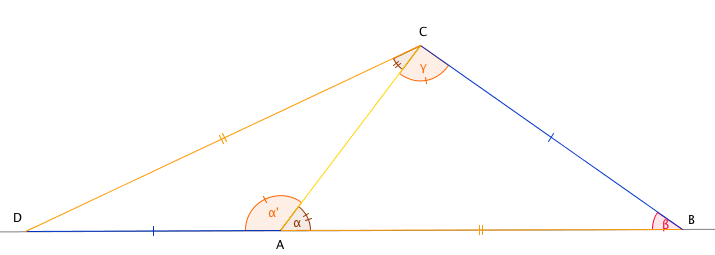
\includegraphics[scale=0.6]{Angle_externe_2.png}
    \end{figure}
	\begin{flushright}
    $\bigstar $
    \end{flushright}
    
    \item Nous considérons le triangle $\triangle abc$ et nous plaçons un point $B'$ sur le segment $AB$, tel que $\angle{ACB'} \equiv \alpha'$.
     Donc ce triangle a un angle externe équivalent à un angle interne, ce qui nous renvoie au premier cas. 
     Il n'est donc pas possible que $\alpha'$ soit plus petit que $\gamma$.
     \begin{figure}[H]
    \centering
    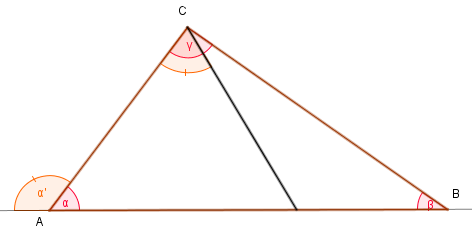
\includegraphics[scale=0.9]{Angle_externe_3.PNG}
\end{figure}
     \begin{flushright}
    $\bigstar $
    \end{flushright}

\end{enumerate}

Nous avons démontré que les cas 1 et 2 sont impossibles et que la seule possibilité est que $\alpha' > \gamma$.
\end{proof}


\end{document}
